\chapter{Introduction}

\section{Space debris}
In this section, we will dive into the topic of space debris. We will explain what it is and what categories there are based on different properties. Next, we will talk about various types of orbits and characterize each one. Finally, we will look at the population of space debris and the trend of its exponential growth. 

\subsection{Definition}
Space debris is defined as all man-made objects orbiting around Earth
that are no longer functional or useful \cite{klinkrad2006space}.
Debris may come in different shapes, sizes, materials and there are various sources of their origin. 

According to \cite{klinkrad2006space}, there are the following types of space debris based on the source of their origin: 
\begin{itemize}
    \item mission-related objects, payloads, and rocket bodies left behind by launches
    \item fragments caused by deliberate or unintentional impacts with other orbiting objects 
    \item non-functional spacecraft, which either failed or served some purpose in past but are now useless
    \item relicts of space activities, like screwdriver left by astronaut or degradation products from coatings of satellites, etc.
\end{itemize}

\subsection{Orbits}

All objects with mass in space are attracted to other nearby objects through gravity. An attracted object follows a curved path around the other object and this path is called the orbit \cite{ESAarticle}.

In the same way, the Moon orbits around Earth, other objects like satellites and space debris also follow a specific curved path with Earth at one focus. We distinguish the following types of orbits, with some of them displayed in the Figure \ref{img:orbits}:

\begin{itemize}
    \item Geosynchronous Earth Orbit (GEO)
    \item Low Earth Orbit (LEO)
    \item Medium Earth orbit (MEO)
    \item Sun-synchronous orbit (SSO)
    \item Geostationary Transfer Orbit (GTO)
    \item Highly Elliptical Orbit (HEO)
\end{itemize}

Objects positioned in GEO are orbiting around Earth above the equator following the direction of Earth’s rotation. Traveling at speed of 3 km per second at an altitude of 35 786 km allows them to match the rotation of Earth and takes about 24 hours to complete one full rotation. 
This fact allows objects to appear 'stationary' over a fixed position, which is suitable for weather or telecommunication satellites. 
A great distance from Earth like this also enables satellites to monitor a large section of the area at once \cite{ESAarticle}.

On the other hand, LEO is the orbit relatively close to Earth, with an altitude of less than 1000km. The typical speed of satellites in LEO is about 7.8 km per second, which means that one full rotation around Earth takes around 90 minutes.
While satellites in GEO are orbiting at the same plane above Earth's equator, the objects in LEO can follow different paths and their orbit planes can be tilted. This allows for more available paths and therefore a more dense population of satellites. 
The proximity of LEO satellites to Earth is convenient for satellite imaging but not much for telecommunication, as they move quickly across the sky and are unable to cover a large area. For this reason, a large combination of satellites is used to provide coverage of the area constantly \cite{ESAarticle}.

MEO consists of orbits between LEO and GEO. Similar to LEO, objects don't need to follow the same path during the orbit around Earth. This is why it's used by satellites with various applications.
One full rotation in MEO ranges from 2 hours to less than 24 hours. 
This orbit is mostly used for navigation or telecommunication purposes, using a combination of multiple satellites to cover the large areas \cite{ESAarticle}.

Unlike other orbits, where satellites travel from west to east, the polar orbit has a path from north to south. A special type of polar orbit is SSO, whose main feature is that satellites are synchronous with the Sun, which means that they stay at the fixed position relative to the Sun. SSO falls into the low Earth orbit, with an altitude ranging from 600 to 800 km from Earth \cite{ESAarticle}. 

There are other orbits like GTO or HEO but these are not that significant when it comes to space debris. 

Distinguishing space debris based on their orbit is yet another useful categorization as this captures their relative position to Earth. 

\begin{figure}[h]
    \centering
    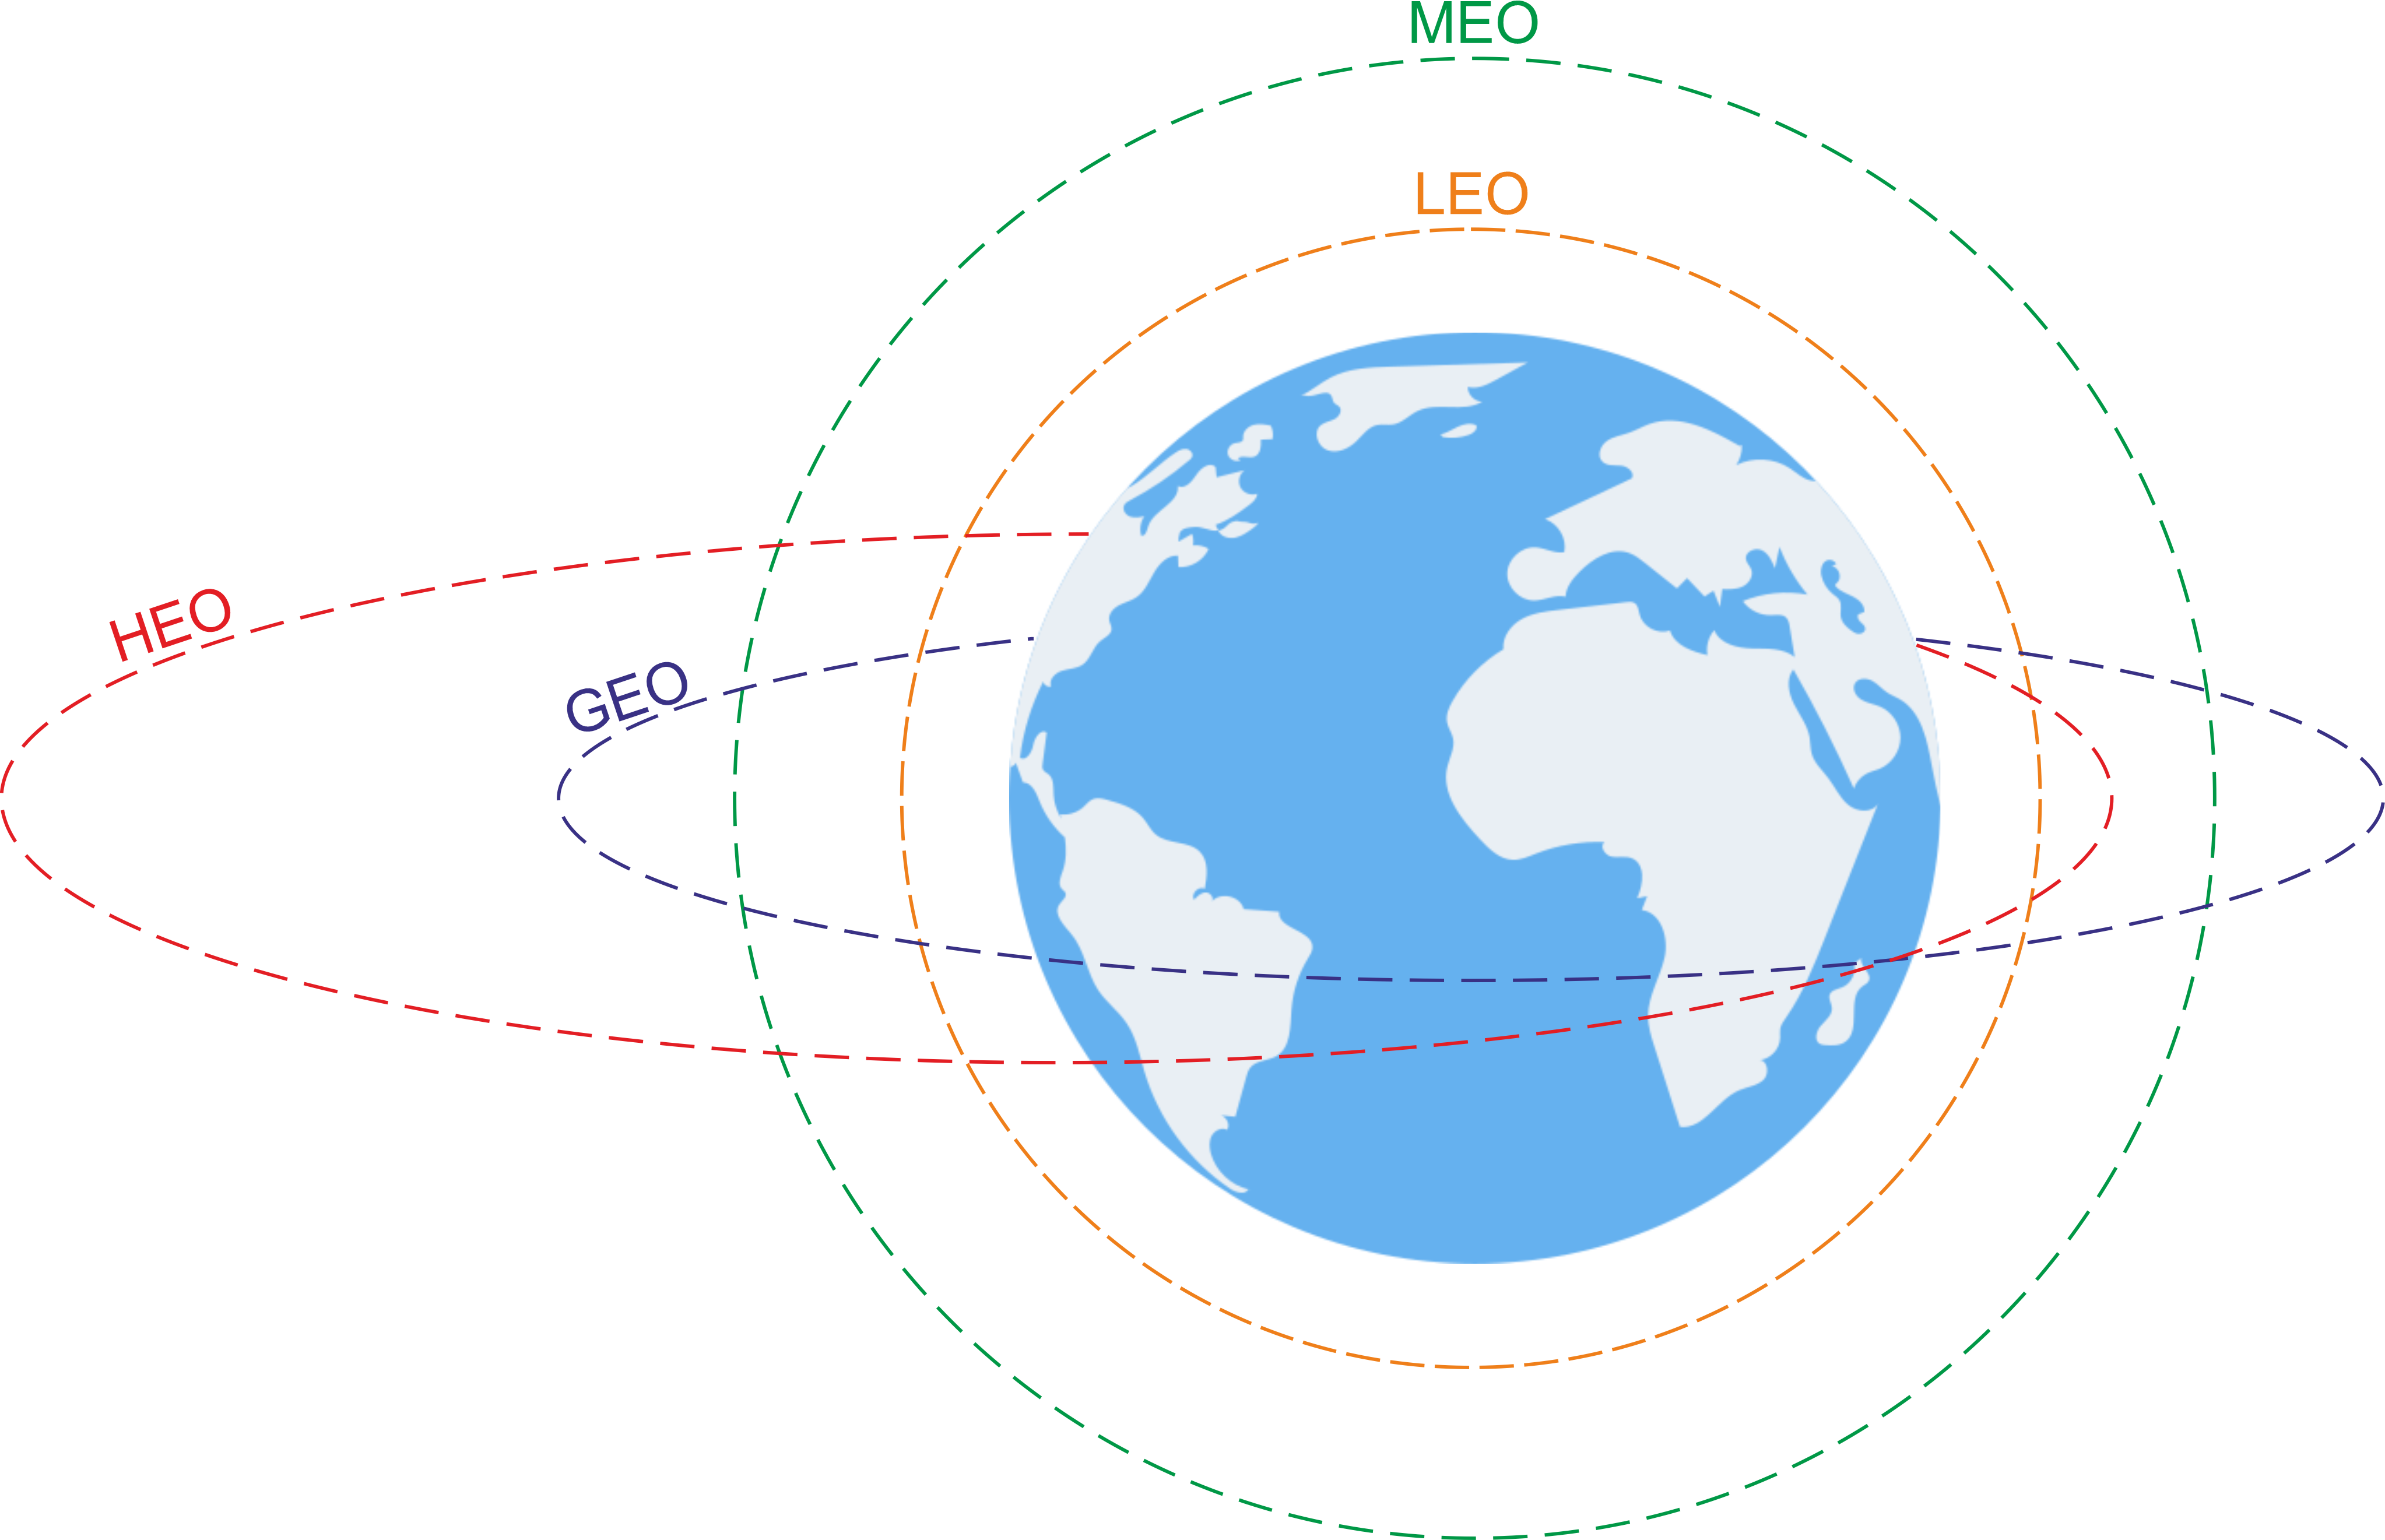
\includegraphics[width=.7\textwidth]{images/orbits.png}
    \caption{Types of orbits.}
    \label{img:orbits}
\end{figure}

\subsection{Population}

For more than 60 years, US Space Surveillance Network (USSSN) maintains a catalog of tracked objects in space. As of March 2022, this catalog contains more than 56 000 objects, from which about 29 000 are space debris \cite{ESAarticle2} \cite{ESAarticle3}.
However, due to the limitations of telescopes and radars, space debris of smaller sizes can not be detected. The minimal detectable size also depends on their orbit as well. In LEO, objects with a size of around 5-10 cm can be observed, while in GEO the minimal threshold is around 30 cm \cite{klinkrad2006space} \cite{ESAarticle2}.
This means that the real amount of space debris is much higher than what is stated in catalogs. According to statistical models, it is estimated that more than 130 million space debris objects with sizes ranging from 1 mm to 1 cm are still in orbit \cite{ESAarticle3}.

In 2002, a study was conducted to estimate the types of objects present in the space. It was based upon 9000 cataloged on-orbit objects. Classifying based on object origin, it was estimated that around 31.8 \% were payloads, 17.6 \% spent rocket upper stages and boost motors, 10.5 \% mission-related objects, and around 40 \% fragmentation debris. 
Considering the orbit, it was estimated that around 69.2 \% of objects were in LEO, at an altitude below 2000 km. This matches the fact that LEO is considered to have the densest population of objects. In contrast, the GEO made up only 9.3 \% of objects, 9.7 \% were in HEO and GTO, 3.9 \% in MEO, and the remainder of  7.8 \% was outside of GEO region \cite{klinkrad2006space}.  

In the Figure \ref{img:esaspacedebrisreport}, we can see the time evolution of tracked on-orbit space debris based on their origin. This shows that the debris population is rising exponentially. Moreover, with the current increasing interest in deployment missions, the amount of space debris will continually follow this trend. And with an increase in space debris, the probability of collisions grows simultaneously. Therefore, regular surveillance and tracking of space debris is very useful for present and future missions, as this could prevent unexpected impacts and ensure better safety \cite{ESAarticle2}. Data from the space debris observations are often acquired with astronomical telescopes which produce astronomical images (see Chapter \ref{chap:astronomicaldata}). 

\begin{figure}[h]
    \centering
    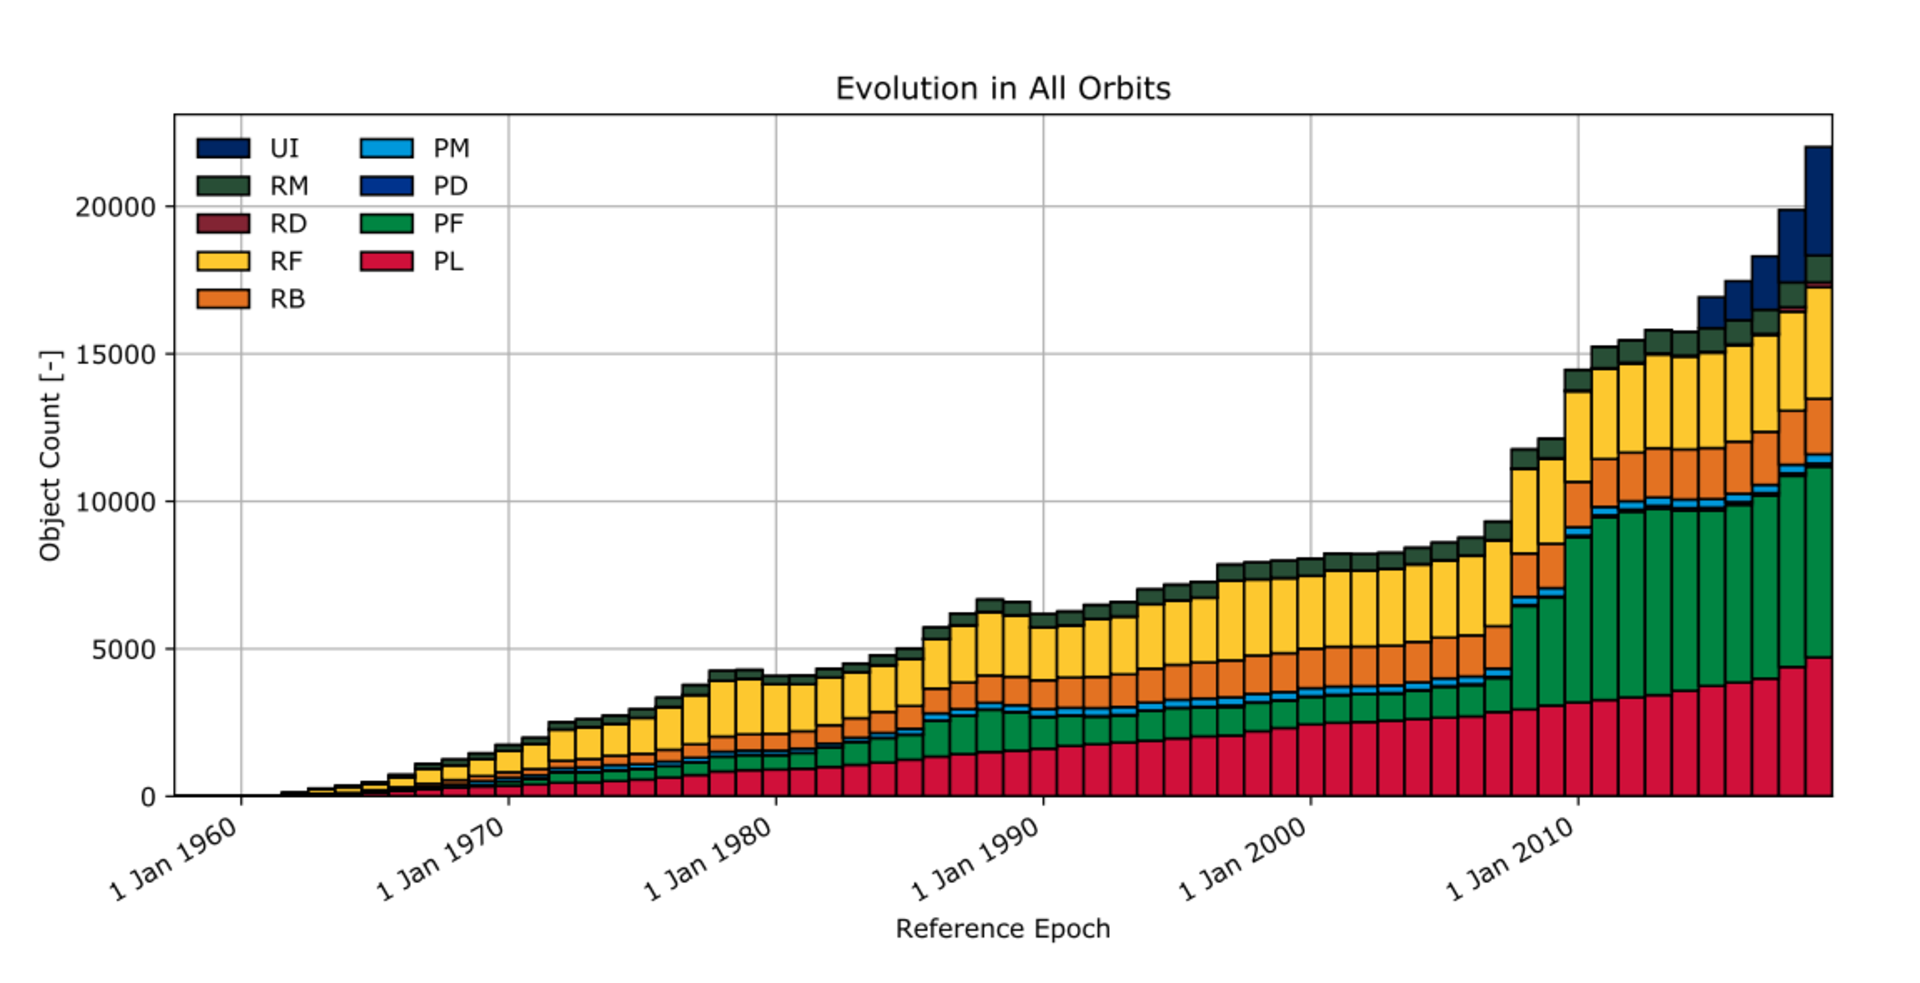
\includegraphics[width=\textwidth]{images/ESA.png}
    \caption[The evolution of number of space debris objects based on different types of objects.]
    {The evolution of number of space debris objects based on different types of objects.
    (UI = Unidentified, RM = Rocket Mission Related Object, RD = Rocket Debris, RF = Rocket Fragmentation Debris, RB = Rocket Body, PM = Payload Mission Related Object, PD = Payload Debris, PF = Payload Fragmentation Debris, PL = Payload) Source: \cite{ESAarticle2}.}
    \label{img:esaspacedebrisreport}
\end{figure}




 
    
    
    
    


\section{Deep learning}
% something about deep learning 
    % convolutional neural network
        % convolutional layers, pooling, FC
    % maybe about resnet if I wanna compare it
    

Solving mathematical problems is a very easy task for computers. However, the real challenge is to solve problems that are natural to humans but cannot be formally described by a set of rules for computers. Things like understanding spoken words, recognizing objects, or identification of people are all instinctively learned by humans and require years of experience. For computers to gain this knowledge, a similar concept is used. They also learn from experience by using a large amount of provided data. The system of learning is based on a hierarchy of concepts, where each concept is built upon relations with simpler concepts. Drawing a graph of this hierarchy would result in a deep structure of concepts, which is where the name deep learning comes from \cite{Goodfellow-et-al-2016}.

In this section, we will talk about a specific type of deep learning technique - convolutional neural networks. 

\subsection{Convolutional neural network}

A convolutional neural network (CNN) is a specific type of neural network that operates on grid-like data. It is most commonly used when working with images, which are represented as a 2D grid of pixel values \cite{Goodfellow-et-al-2016}.

The process is the same as with a neural network, but the inner structure is different. The CNN receives the input, which is fed through the series of hidden layers and the final score is computed in the output layer. Each layer is made up of a set of neurons, which have learnable weights and biases. However, the neurons in CNN are arranged in 3 dimensions: width, height, and depth as is depicted in the Figure \ref{img:cnn0}.

\begin{figure}[h]
    \centering
    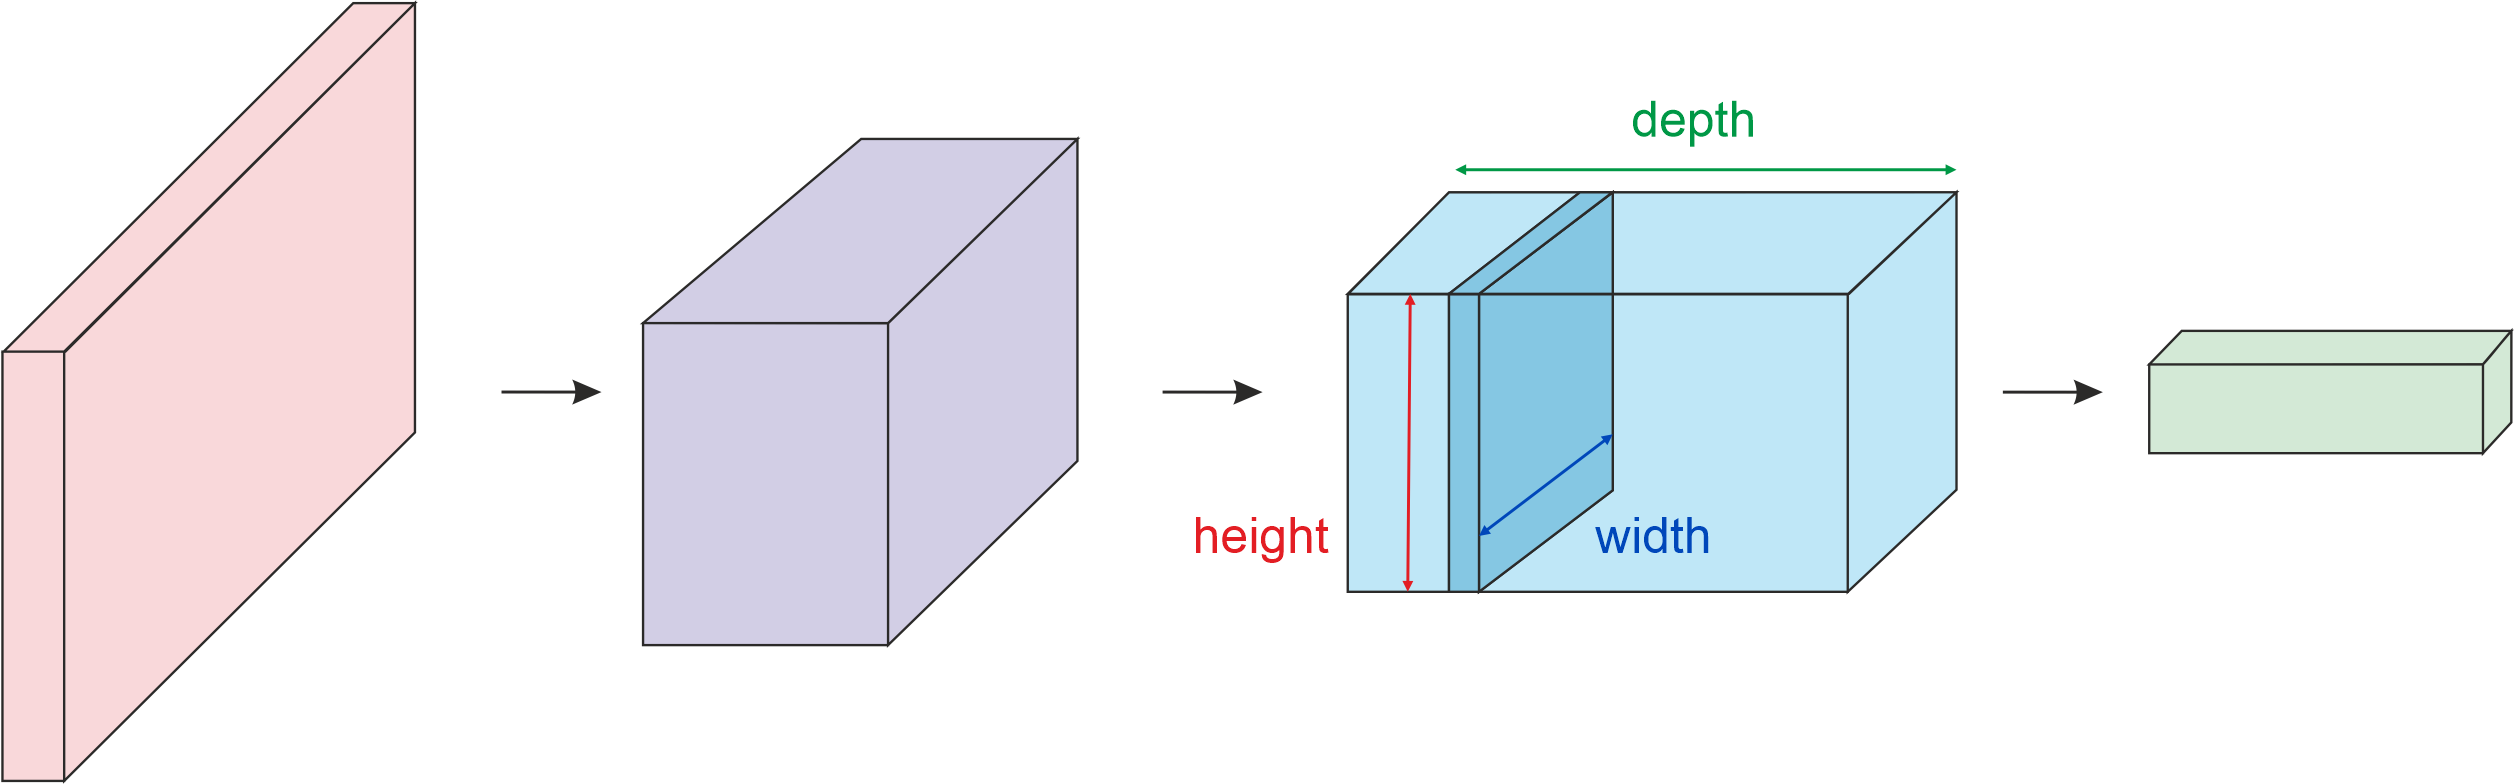
\includegraphics[width=.8\textwidth]{images/cnn.png}
    \caption{Inside structure of convolutional neural network.}
    \label{img:cnn0}
\end{figure}

%In neural networks, layers are fully connected, which means that each neuron from the previous layer is connected to each neuron in the following layer. 

While in neural networks, all layers are fully connected, the CNN has 3 main building blocks: convolutional layer, pooling layer, and fully connected layer \cite{standford}.

\subsubsection{Convolutional layer}

The convolutional layer is the most essential part of CNN and as the name suggests, this is where the convolution operation happens. Each convolutional layer has a defined set of filters/kernels. The filter has a significantly smaller spatial size than the input image (ranging from 3 to 10 pixels wide) but covers the full depth of the input. The values of each filter represent weights learned by the network \cite{standford}.

During the forward pass of the network, the convolution is applied to the input volume in a manner that each filter is moved across the width and height of the input. How many pixels the filter moves during convolution is defined by parameter stride. At each position, a dot product is computed between values of the filter and values of the input. This creates a 2D activation matrix also called a feature map. 
This way, each filter in the layer creates a feature map containing the response of that specific filter at each spatial position of the input. Stacking all these feature maps together builds the output volume of the layer, where the depth is the number of filters in the layer \cite{Goodfellow-et-al-2016} \cite{standford}.

Formally, the convolution is defined by the following formula:
\begin{equation}
    (K * I) (i,j) = \displaystyle\sum_{m}  \displaystyle\sum_{n} I(i - m, j - n) K(m, n).
\end{equation}
where K is the kernel, and I is the input volume \cite{Goodfellow-et-al-2016}.

A simple example of convolution applied to 2D input is shown in the Figure \ref{img:conv0}. It shows how the kernel is moved through the matrix with a stride 1 and how the dot product at each position is calculated. 

\begin{figure}[h]
    \centering
    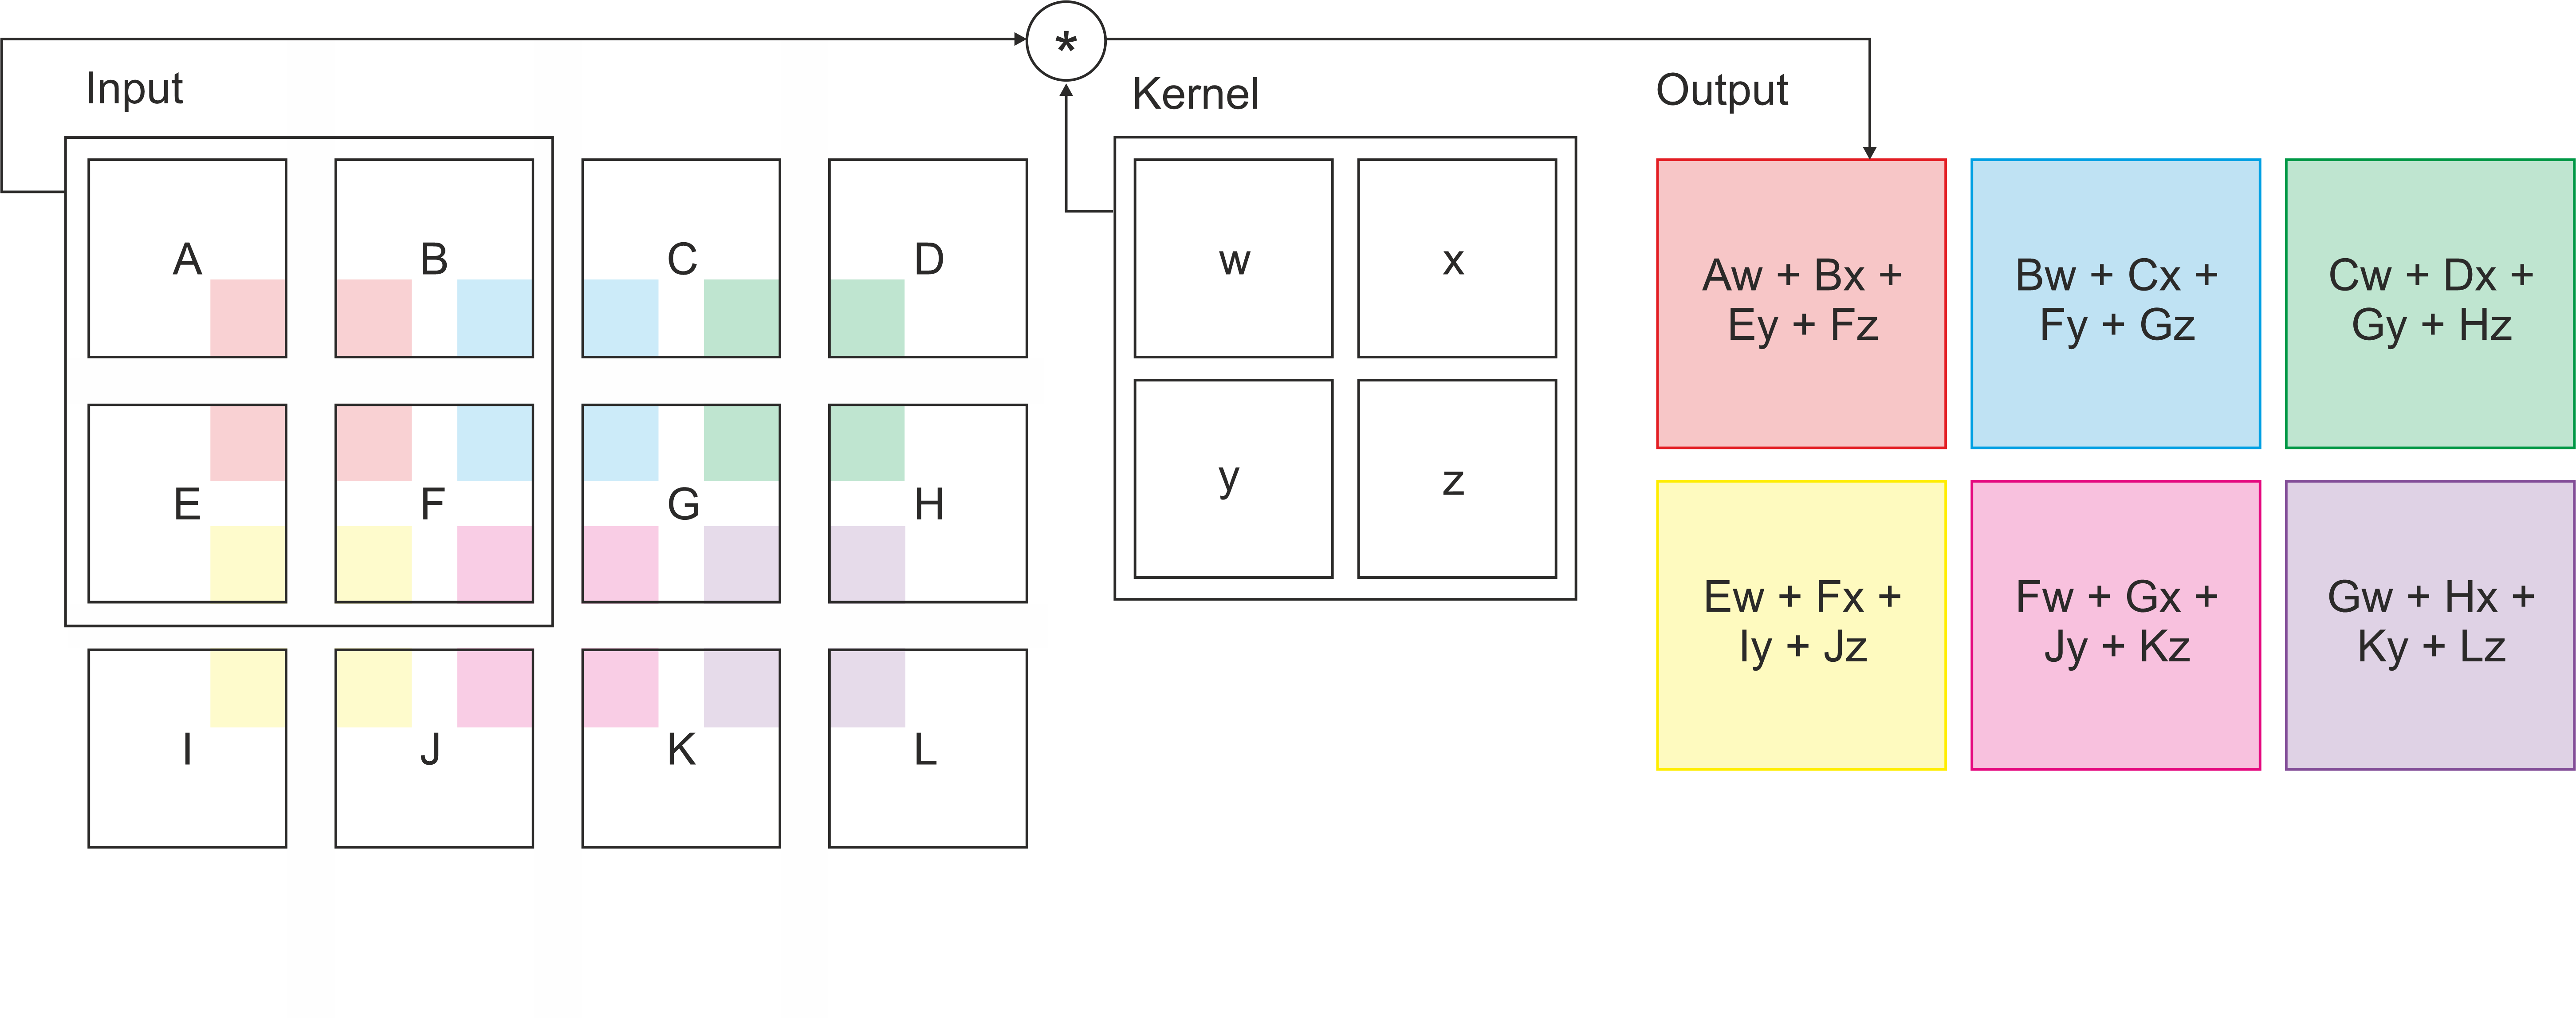
\includegraphics[width=.8\textwidth]{images/convolution3.png}
    \caption{An example of simple convolution.}
    \label{img:conv0}
\end{figure}

\subsubsection{Pooling layer}

Another important layer in the architecture of CNN is the pooling layer. It is useful for reducing the spatial size of feature maps and therefore makes the computation more effective as the network gets deeper. It is also helpful in keeping the representation approximately the same when the input image is slightly translated \cite{Goodfellow-et-al-2016}.

The pooling layer has a defined size of the kernel, which usually ranges from 2x2 to 3x3 pixels spatially. Another important parameter is the pooling function that is performed on the input. The most common is max pooling, but there are other popular pooling functions such as average, weighted average, or L2 norm pooling. 
Unlike other layers in the CNN, the pooling layer has no learnable parameters \cite{standford}.

Pooling is performed in a similar fashion as convolution. A kernel is moved across the input volume spatially but operates on each depth slice separately. This way only the spatial size of the input is reduced and the depth stays the same. At each spatial location, the output value is computed using the pooling function performed on the values of the input \cite{standford}.

The process of max pooling is illustrated in the Figure \ref{img:maxpool0}. The size of the kernel in the example is 2x2 with a stride of 2. It is common practice to use the stride the same size as the kernel if we do not want an overlapping pooling.  

\begin{figure}[h]
    \centering
    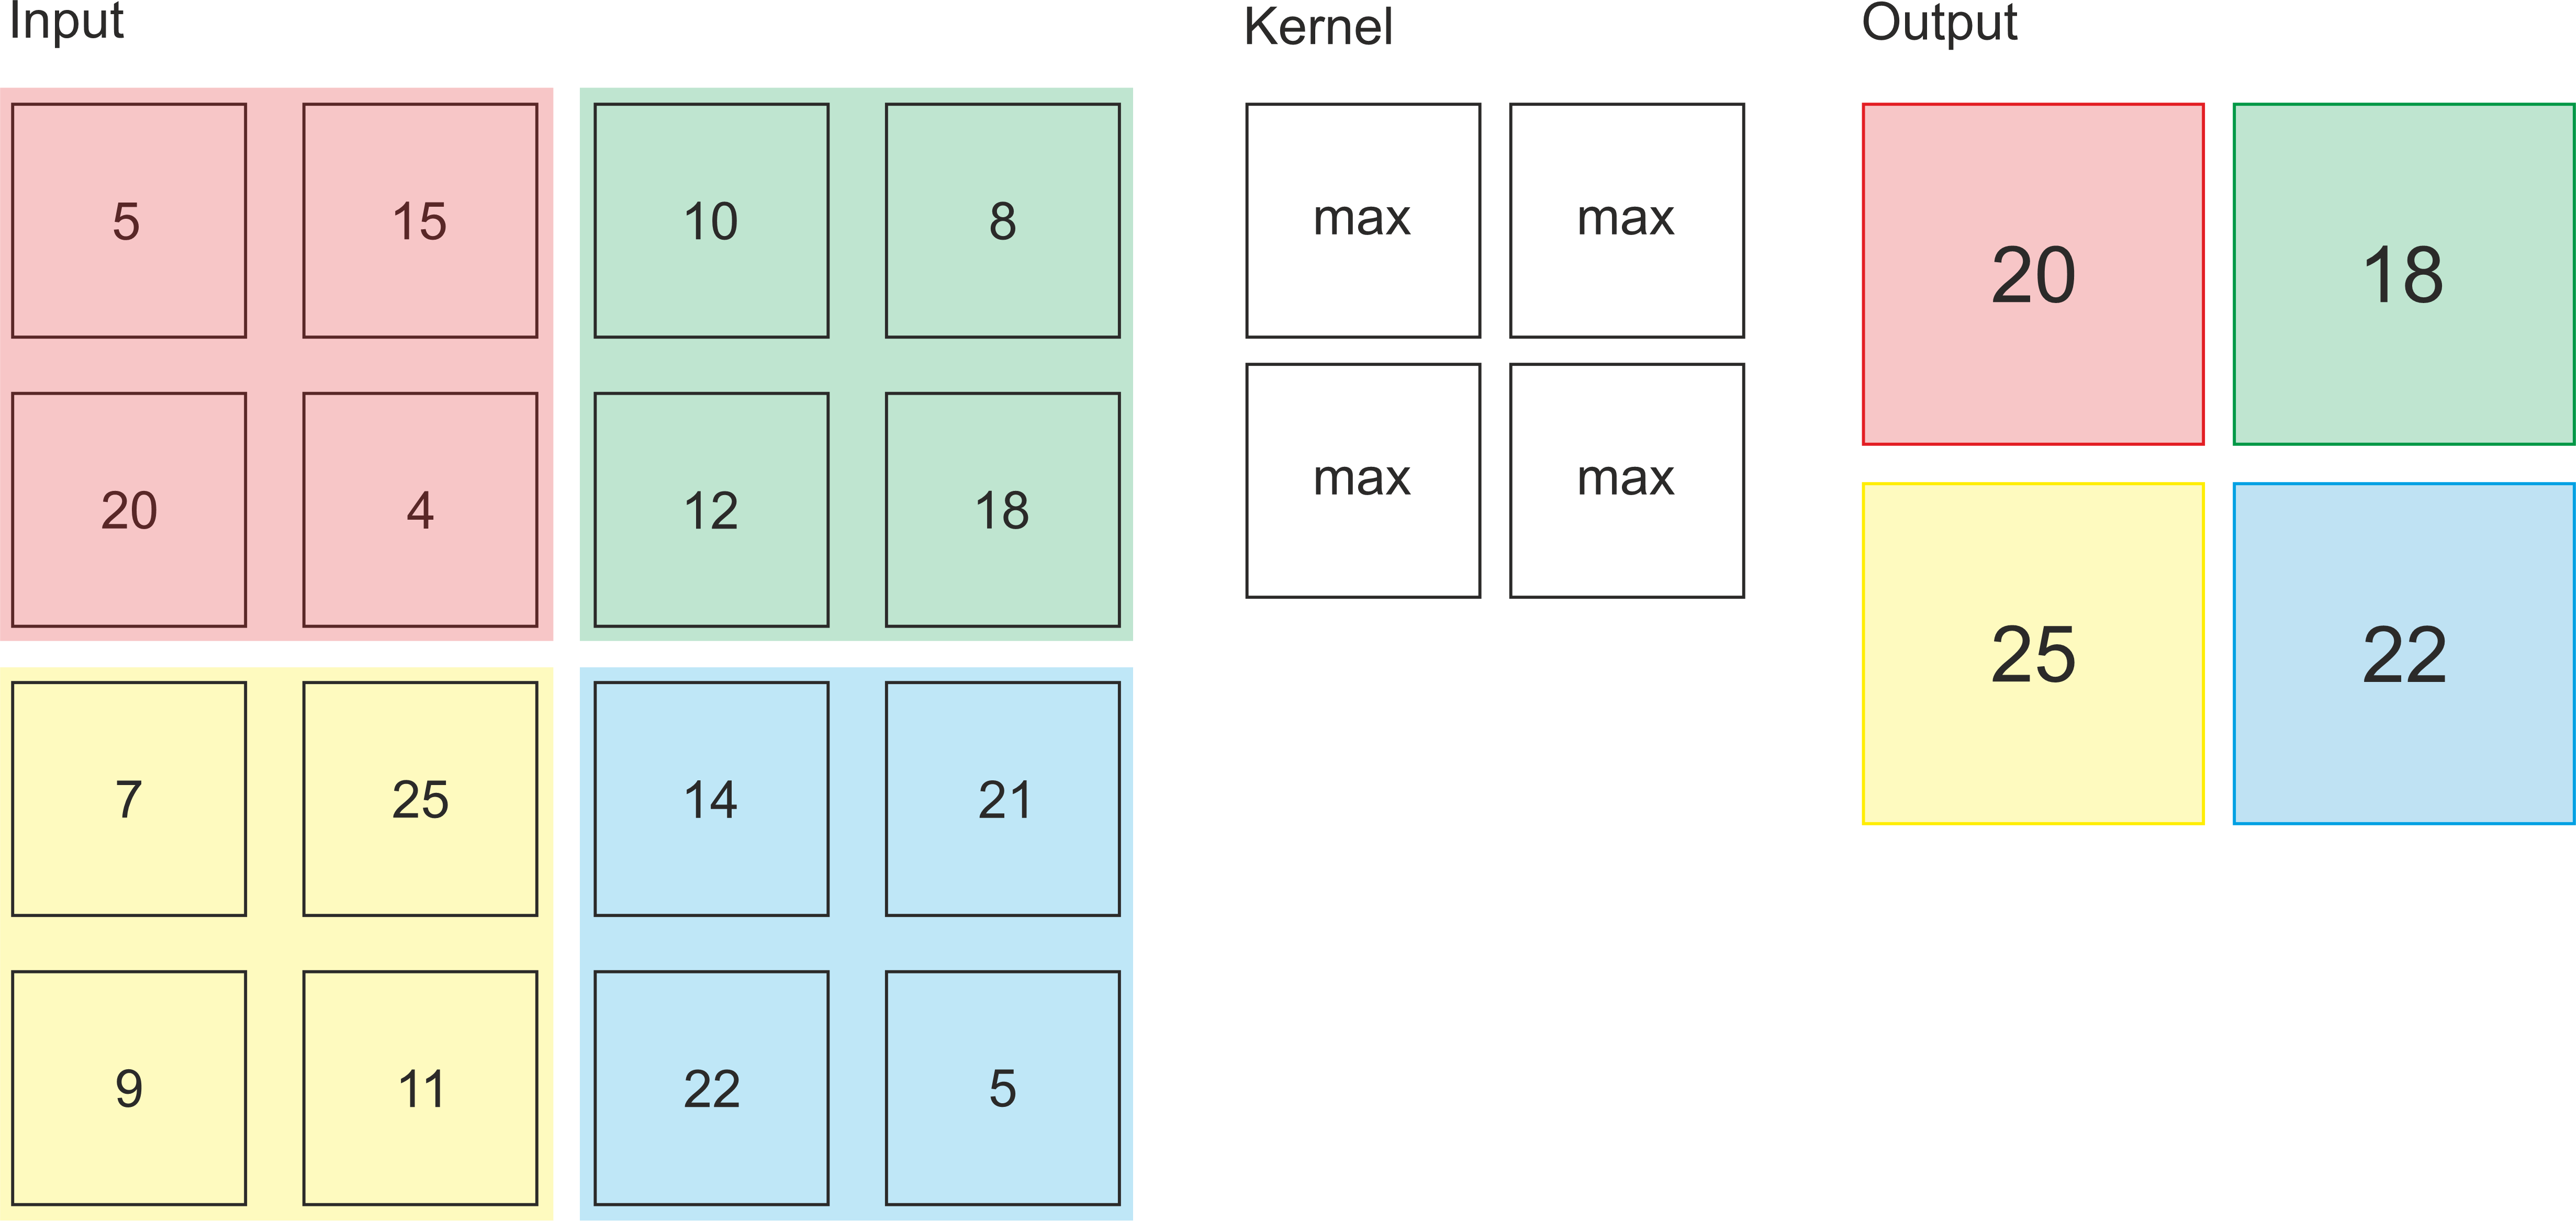
\includegraphics[width=.7\textwidth]{images/maxpooling.png}
    \caption{An example of max pooling.}
    \label{img:maxpool0}
\end{figure}

\subsubsection{Fully-connected layer}
Fully connected (FC) layers in CNN are identical to layers in a standard neural network. They consist of neurons that have no connection to each other within one layer, but each neuron from the previous layer is connected to each neuron in the following layer \cite{Goodfellow-et-al-2016}.

The structure of neurons in FC layers is no longer organized in 3 dimensions instead inputs and outputs are 1D vectors. Feature maps fed to a fully-connected layer, therefore, need to be flattened to one dimension.

While in standard neural networks, each layer is fully-connected, in CNN only the last layers that are responsible for calculating the class scores are fully-connected \cite{standford}.

\section{Space object recognition} \label{sec:spacerecognition}
Object recognition refers to a series of computer vision tasks, whose goal is to identify objects on images. It consists of two separate tasks: object localization and classification. 
The first step of object recognition is to find all objects present in the image, which is the goal of the object localization task. The algorithm outputs the location of the object as well as the bounding box encapsulating the object. Each object is then assigned a label that defines the class that the object belongs to. This is called classification. 
%Next, features from each object need to be extracted. This can be done by means of traditional or deep learning methods. Based on these features, each object is assigned a label that defines the class that the object belongs to. This is called classification. 

%Object recognition is used in many areas of life. 
%% nieco kde sa to pouziva a potom ze sa to pouziva aj v astronomical field

In this chapter, we will talk about various approaches to object recognition through astronomical images or features extracted from them. %We will focus on two main things: the type of data and the proposed method. 

\subsection{Traditional methods}
For many years traditional analytical methods were used for object recognition. These methods relied on astronomers‘ knowledge of the given task and were designed for specific types of space objects. 

\subsubsection{On-orbit recognition of resident space objects by using star trackers}
The main goal of the article \cite{SPILLER2020478} was to evaluate the possibility of using star trackers to track resident space objects (RSO) in space. For this purpose, they developed an algorithm that could operate on board with limited computational performance and memory.
With this in mind, the algorithm could not be based on machine learning as this would be computationally demanding. 

In order to test the proposed algorithm, synthetic images needed to be generated using their own star-tracker hardware simulator. 
The simulator consists of two modules:
\begin{itemize}
    \item Sky and spacecrafts input generator
    \item High-fidelity image generator

\end{itemize}

The goal of the first block is to simulate the sky, stars, and RSOs. The sky simulation is performed using a star catalog while considering the position and orientation of the sensor as well as optical and geometric characteristics. A similar procedure is followed when simulating real RSOs, but using the catalog with orbiting RSOs instead of the star catalog. Another way of simulating RSOs is to use the grid method, which simulates fictitious RSOs. 
The second block is used to make the image realistic. The block receives the list of stars and RSOs with their position and magnitude. Using this data as well as some additional information regarding noises, optical, geometrical, and electronic characteristics of the sensor, the block produces high fidelity synthetic images. 

When it comes to the developed algorithm, the first step is to identify objects of interest from the background. After the identification of objects is complete, a list of objects and their positions is produced for every image. 
The algorithm is then given pairs of images and compares each object on the first image to each object in the second image. Based on some predetermined conditions regarding their position, distance, velocity, and density, objects are matched. This means that the object in the first image is the same object in the second image. The algorithm performs this comparison for a series of pairs of images and as a result, the object is being tracked.

This method was mainly developed to track moving objects in space-based observations. In this situation, RSOs usually appear as streaks and the algorithm was optimized for this scenario. However, this poses a disadvantage since point-like objects are not recognized well and diffuse sources are considered background noise. 

\subsection{Machine learning methods}
With an increase in the amount of data, the traditional methods weren't fast and robust enough. Machine learning methods were able to tackle this issue, by learning on their own. Extracting knowledge from a large amount of data allows them to find patterns in data that may not be visible to humans. This way they can outperform even the best traditional methods \cite{Goodfellow-et-al-2016}.

 
\subsubsection{Galaxy morphology classification using automated machine learning} 
In \cite{REZA2021100492}, multiple machine learning algorithms were tested with an aim to classify galaxies into four types. The study was conducted in order to assess the possibility of using ML for future surveys. 

Dataset used to train models contained more than 304 000 samples of galaxies of different types (spirals, ellipticals, mergers, and stars). Feature vectors were obtained from SDSS (Sloan Digital Sky Survey) and their extraction wasn't explained since that is not the main subject of the article. %Feature vector included features such as fiber, model and Petrosian colors, axis ratio, degree of ellipticity, and others. Explanation of each feature is provided in the mentioned article \cite{REZA2021100492} and will not be done here since they are not relevant to this thesis. 

Five different ML methods were chosen for the article - Decision trees, Random Forest, ExtraTrees, K-nearest neighbors, and Artificial Neural Network. Before the data was fed to any model, PCA was performed on feature vectors to reduce their dimensionality. As a result, 25 most significant features were used from the original feature vector of size 62. As usual, models were trained on the training set and hyperparameters were tuned on the separate validation set. 
Evaluating the models on the testing set and comparing the accuracy showed that ANN had the best results. Even though the overall accuracy of the ANN was the best, the accuracy of minority class samples showed poor results. In this case, ensemble methods like a combination of ExtraTrees with Random Forest performed much better. In conclusion, we can say that using a balanced dataset with a large number of samples could prove to be useful when working with ANN. 




\subsubsection{Applications of neural networks to object detection and star/galaxy classification}
%https://academic.oup.com/mnras/article/319/3/700/1073630?login=false
In the article, \cite{Andreon2000}, the developed package called Neural extractor (NExt) was presented. The package can perform object detection and star/galaxy classification. The authors used three different NNs for each specific task: data reduction, detection, and classification. 

For the training, validation, and testing, the subset of the IP92 catalog \cite{1992ApJS} was used. To train the detection part of the algorithm, the best solution was to use around 10 subimages 50x50 pixels wide. To test the performance of the detection and classification networks, 4819 and 460 objects from the catalog were chosen, respectively.

The first step of the package included the detection of desired objects. This task was performed as a classification of pixels into background and object class. First, the non-linear PCA NN was applied to the image, which reduced the redundant information in nearby pixels. Transformed values of the pixels were then fed to unsupervised NN. Multiple different models were tested and the best performing one was a multi-layer neural gas network with a running window of size 3 or 5. 
This network aimed to classify pixels into background or object class. This was done in an unsupervised matter and the network has split pixels into multiple classes. One of the classes could be described as a background, whereas the others described different kinds of astronomical objects and were later merged to form an object class. After the segmentation, the overlapping objects were detected and deblended.
The second step included feature extraction and the star/galaxy classification. Considering feature extraction, multiple features were measured, and through the sequential backward elimination strategy, the best-performing ones were selected. These features were then used to train MLP to perform the final task of star/galaxy classification. 

To test the performance of the proposed method, the authors compared the results to the best performing package at the time (SExtractor \cite{sextractor}). Considering the detection phase of the algorithm, the proposed method was as effective as the SExtractor in the detection of true objects. For the classification phase, the NExt performed better than the SExtractor, with only 28 errors compared to 41 for the SExtractor from the total of 480 objects. 

It wasn't explicitly mentioned in the article but according to pictures, this method considers the only point-like appearance of the stars. This poses a huge disadvantage in our case since the space debris usually appears as streaks during the sidereal tracking.  



\subsubsection{Deblending and classifying astronomical sources with Mask R-CNN deep learning}
In \cite{Burke2019}, a network based on Mask Region-based CNN (Mask R-CNN) framework is used to detect, classify and deblend star and galaxy sources. 

The network is trained, validated, and tested using simulated images generated by The Photon Simulator. The simulator generates 512x512 three-band images, where each image contains around 150 objects. For the training set, 1000 images were simulated, which is approximately 150 000 astronomical sources. The validation and testing set contains 250 and 50 simulated images, respectively. 

The Mask R-CNN \cite{maskrcnn2017} comes from a family of region-based CNN frameworks, that specialize in the task of object recognition. The architecture of the R-CNN framework could be summarized as multiple subnetworks, where each has its own specific task. The backbone of the framework is a deep CNN, whose goal is to extract features from the image. The region proposal network finds regions in the image and the type of object in the area. At the end of the framework, there are 2 subnetworks, one predicts the type of object in the proposed region, and the other outputs the bounding box of the object. Mask R-CNN is an extension of R-CNN frameworks, with additional subnetwork for instance segmentation.
In the article, the backbone used for Mask R-CNN is a Resnet with 101 layers. Transfer learning was used to improve the speed of the training process, with initial weights trained on the MS COCO dataset.  

The network was tested on simulated images and achieved a precision of 92 \% on star sources and 98 \% on galaxies. Results also revealed that the network performs significantly better with small sources, which could be due to a few large examples in the training set. 





%%%%%% does not need to cite

% articles about streaks
% https://cds.cern.ch/record/1707548/files/978-1-4939-0629-1_BookBackMatter.pdf
% https://conference.sdo.esoc.esa.int/proceedings/neosst1/paper/444/NEOSST1-paper444.pdf
% https://www.aanda.org/articles/aa/full_html/2020/12/aa37765-20/aa37765-20.html
% https://reader.elsevier.com/reader/sd/pii/S0094576521001211?token=93F8903DF4BF28EC64C9DE8B86B59D6C71136A835A32EB40977BA9A729EB5DAFCCF2437D4B81A5717C58E2BC46B52704&originRegion=eu-west-1&originCreation=20210804182521

% articles about astronomical imagining
% https://link.springer.com/chapter/10.1007/978-3-319-21969-1_37
% https://subarutelescope.org/staff/guyon/15teaching.web/00AstrOptics.web/AstrOpt_01fund.pdf

% articles about ccd artifacts
% https://arxiv.org/pdf/1601.07182.pdf
% https://mwcraig.github.io/ccd-as-book/01-00-Understanding-an-astronomical-CCD-image.html

% articles about noises
% https://hamamatsu.magnet.fsu.edu/articles/ccdsnr.html
% https://www.mssl.ucl.ac.uk/www_detector/ccdgroup/optheory/darkcurrent.html
% https://camera.hamamatsu.com/jp/en/technical_guides/calculating_snr/index.html






